\chapter{Projektformulering og afgrænsning}
I daglig klinisk praksis er der ofte behov for kontinuert at monitorere patienters blodtryk, i særdeleshed på intensive afdelinger samt operationsstuer, hvor blodtrykket er et vigtigt parameter til monitorering af deres helbredstilstand. \\
Blodtrykket måles invasivt, det vil sige, at Blodtryksmålesystemet er tilsluttet patienternes arterier via et væskefyldt kateter, som afbildet i Figur 2.1.
\begin{figure}[H]
	\centering
	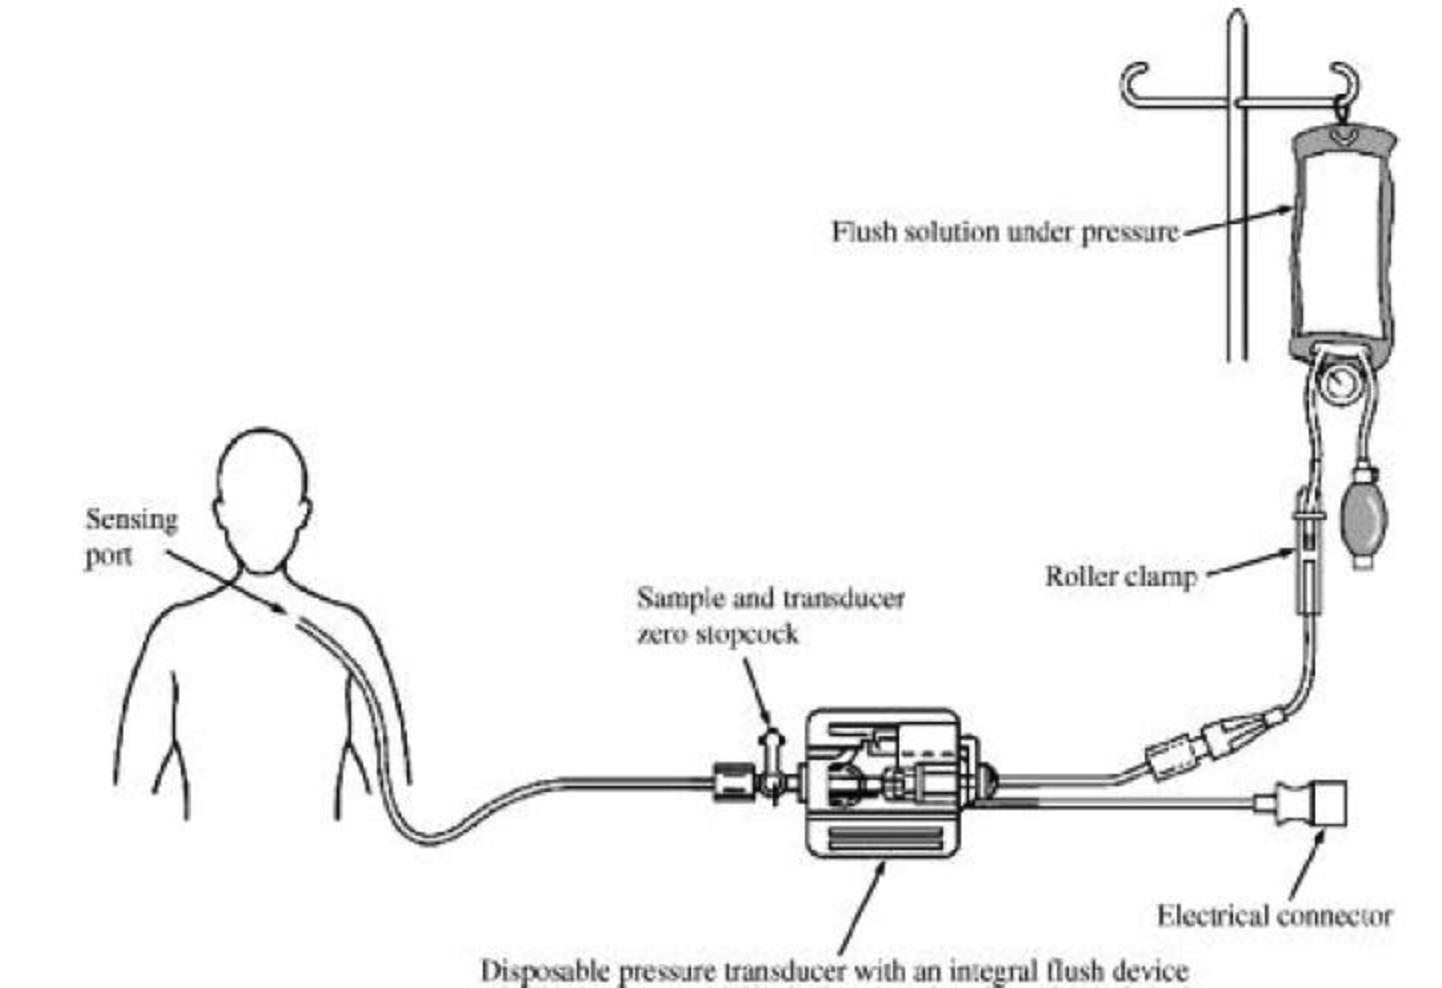
\includegraphics[width=1\textwidth]{Figurer/Snip20151207_50}
	\caption{Måleopstilling, \protect\cite[s. 296]{Billed for invasiv blodtryksmaling}}
\end{figure}

I dette projekt bliver der fokuseret på at udvikle et blodtryksmålesystem, som kan benyttes til forskning, hvor det typisk vil være interessant at observere blodtrykket kontinuerligt.
Systemet realiseres ved udvikling af to elementer, hvoraf det ene består af et elektronisk hardwarekredsløb, hvis formål er at forstærke signalet fra en tryktransducer samt at filtrere signalet med et indbygget analogt filter.\\
Det andet element realiseres ved et C\#-program, der skal udskrive blodtrykket som funktion af tiden. Programmet skal derudover leve op til en række krav for blandt andet kalibrering, nulpunktsjustering, digital filtrering samt mulighed for at gemme interessante målinger af blodtrykssignalet til efterfølgende forskning i en database.
Ydermere er der valgt at afbildede systolisk og diastolisk blodtryk med tal, samt angivelse af pulsværdi.\\\\
I forhold til udvikling af softwaren, har det været nødvendigt at lave antagelser, hvad angår design af brugergrænsefladen, da der ikke har været kommunikation eller mulighed for test af systemet med slutbrugerne. 

\subsubsection{Ansvarsområder}
De forskellige opgaver i forhold til udvikling af Blodtryksmålesystemet er blevet uddelt mellem gruppemedlemmerne. Der er en gruppe, der har haft ansvaret for udviklingen, dokumentationen samt rapportelementer for hardwaren, mens den anden gruppe har haft ansvaret for udviklingen, dokumentationen samt rapportelementer for softwaren. Alle gruppens medlemmer har haft ansvaret for de resterende rapportelementer. Opdelingen kan ses i Tabel 2.1.    

\begin{longtabu} to \linewidth{@{}l  X[j]@{}}
	\textbf{HW udvikling og dokumentation} & \textbf{SW udvikling og dokumentation} \\[-1ex]
	\midrule
	Lise Skytte Brodersen & Anders Wiggers Birkelund\\[-1ex]
	Nina Brkovic & Toke Tobias Aaris \\[-1ex]
	Annsofie Randrup Wagner & \\[-1ex]
	Jakob Degn Christensen & \\[-1ex]

	\caption{Ansvarsområder}
\end{longtabu}



